\chapter{Hiện thực ứng dụng webfuzzer}
Chương này mô tả chi tiết hiện thực của kiến trúc hệ thống ứng dụng webfuzzer, bao gồm ba thành phần backend, \acrshort{ui} và cơ sở dữ liệu của ứng dụng.
\section{Backend}
Đề mục này trình bày chi tiết hiện thực backend của ứng dụng webfuzzer, bao gồm giao diện lập trình ứng dụng, định dạng dữ liệu của phần mở rộng Burp Suite, các biến môi trường, cấu hình và mô-đun kiểm thử, theo thiết kế đã đề ra ở \textbf{Chương 5}.
\subsection{Giao diện lập trình ứng dụng}
Backend của ứng dụng webfuzzer sẽ làm việc rất nhiều với cơ sở dữ liệu MySQL. Chúng tôi hiện thực các hàm kết nối cơ sở dữ liệu, truy vấn và mở/đóng kết nối sau quá trình thực hiện câu truy vấn, định dạng dữ liệu trả về từ database cũng như các phương thức liên quan đến giao dịch (transaction) trong tập tin \texttt{services/db.js} trong thư mục gốc mã nguồn backend để tiện quản lý và sửa đổi nhất quán.\par
Những \acrshort{api} liên quan đến việc truy vấn danh sách request mẫu và thông tin yêu cầu kiểm thử đều được hỗ trợ thêm các thuộc tính \texttt{limit, offset} và \texttt{total} để truy vấn một khoảng dữ liệu xác định, phục vụ quá trình phân trang các dữ liệu này ở giao diện người dùng như Đoạn mã \ref{lst:sql-query-with-paging} sau.
\begin{lstlisting}[style=ES6, label={lst:sql-query-with-paging}, caption={\acrshort{api} truy vấn danh sách request mẫu có hỗ trợ phân trang}]
let endpointList = await mySqlConnection.query(`SELECT * FROM Endpoint ORDER BY Id DESC LIMIT ? OFFSET ?;`, [limit ? parseInt(limit) : 10, offset ? parseInt(offset) : 0]);
if (endpointList.error) return reject(endpointList.error);
endpointList.results = endpointList.results.map(ele => {
    return { ...ele, BaseRequest: JSON.parse(escapeTarget(ele.BaseRequest)) };
})
let total = await mySqlConnection.query(`SELECT Count(Endpoint.Id) as total FROM Endpoint;`);
return resolve({ endpointList: endpointList.results, total: total.results[0].total });
\end{lstlisting}
Định dạng kết quả trả về của cái \acrshort{api} được quy định bởi Đoạn mã \ref{lst:API-result-format} sau. Nếu có lỗi trong quá trình gọi \acrshort{api} thì \acrshort{http} response phản hồi có mã lỗi 400 cùng với thông tin về lỗi trong trường \texttt{error}, ngược lại trong trường hợp gọi \acrshort{api} thành công thì response phản hồi có mã lỗi 200 cùng với dữ liêu cần truy vấn trong trường \texttt{results}.
\begin{lstlisting}[style=ES6, label={lst:API-result-format}, caption={Định dạng kết quả API trả về ở backend}]
const response = (res, result, error) => {
  res.status(error ? (error.httpCode || 400) : (result ? result.httpCode || 200 : 404)).send({ 'error': error, 'results': result });
}
\end{lstlisting}
\subsection{Phần mở rộng Burp Suite}
Phần mở rộng Burp Suite cho phép gửi \acrshort{http} request mẫu từ mô-đun \texttt{Intruder} của Burp Suite đến công cụ \textbf{webfuzzer} theo định dạng JSON như Đoạn mã \ref{lst:base-request-format} dưới đây, quá trình chọn và gửi request mẫu sẽ được trình bày ở \textbf{Phụ lục A} của luận văn.
\begin{lstlisting}[style=ES6, label={lst:base-request-format}, caption={Cấu trúc của một HTTP request mẫu được gửi từ phần mở rộng Burp Suite}]
{
  "url": "http://testphp.vulnweb.com:80/showimage.php?file=\xa7./pictures/1.jpg\xa7",
  "cookies": "",
  "headers": {
      "User-Agent": "Mozilla/5.0 (X11; Ubuntu; Linux x86_64; rv:74.0) Gecko/20100101 Firefox/74.0",
      "Accept": "text/html,application/xhtml+xml,application/xml;q=0.9,image/webp,*/*;q=0.8",
      "Accept-Language": "en-US,en;q=0.5",
      "Accept-Encoding": "gzip, deflate",
      "DNT": "1",
      "Connection": "close",
      "Upgrade-Insecure-Requests": "1"
  },
  "method": "get"
}
\end{lstlisting}
Chuỗi ``\texttt{\textbackslash xa7}'' trong trường \texttt{data.searchFor} biểu thị kí tự ``\$'' trong request mẫu. Các kí tự này thường nằm ở trường \texttt{data} hoặc \texttt{url} trong đoạn dữ liệu JSON để đánh dấu những vị trí chèn payload để ứng dụng web xử lí. 
\subsection{Thiết lập các biến môi trường}
Các biến môi trường (environment variables) được thiết lập để điều chỉnh hành vi của backend ứng dụng webfuzzer một cách linh hoạt mà không cần phải sửa đổi mã nguồn chương trình. Các biến này thường quy định luồng xử lý và các giá trị khởi tạo của chương trình, việc định nghĩa các biến môi trường một cách hợp lý giúp chương trình trở nên uyển chuyển hơn. Trong backend của ứng dụng webfuzzer, giá trị mặc định của chúng được chứa trong tập tin \texttt{globalConfig.js} trong thư mục gốc của mã nguồn. Người dùng có thể sửa đổi theo nhu cầu và khởi động lại backend để áp dụng các giá trị mới. Bảng \ref{tab:env-variables-backend} dưới đây mô tả chức năng của các biến môi trường.
\FloatBarrier
\begin{table}[ht]
    \centering
    \caption{Danh sách các biến môi trường ở backend ứng dụng webfuzzer}
    \label{tab:env-variables-backend}
    \begin{tabular}[ht]{ccl}
        \toprule[1pt]\midrule[0.3pt]
            \textbf{Tên biến môi trường}&\textbf{Kiểu dữ liệu}&\textbf{Mô tả}\\ 
        \midrule
            SERVICE\_PORT&Integer&Cổng khởi chạy backend của ứng dụng\\
            \addlinespace
            {}&{}&Các thiết lập để kết nối đến dịch vụ MySQL\\
            mysqlConfig&Object&của hệ điều hành, bao gồm host:port, tên\\
            {}&{}&cơ sở dữ liệu và thông tin đăng nhập\\
            \addlinespace
            defaultFuzzConfig&Object&Cấu hình kiểm thử mặc định của ứng dụng\\
            \addlinespace
            defaultVulnTypes&Array&Các lỗ hổng cần kiểm thử đối với trường hợp\\
            {}&{}&tự động tạo yêu cầu kiểm thử\\
            \addlinespace
            fuzzStrategy&String&Chiến thuật kiểm thử mặc định của ứng dụng (\texttt{Sniper})\\
            \addlinespace
            autoCreateFuzzRequest&Boolean&Tự động tạo yêu cầu kiểm thử sau khi nhận \acrshort{http}\\
            {}&{}&request mẫu từ Burp Suite với các lỗ hổng mặc định\\
            \addlinespace
            autoFuzz&Boolean&Tự động thực thi yêu cầu kiểm thử vừa tạo nếu\\
            {}&{}&không có yêu cầu nào khác đang được thực thi\\
            \addlinespace
            autoExecuteQueuedRequest&Boolean&Tự động thực thi một yêu cầu kiểm thử đã tạo\\
            {}&{}&ngay khi thực thi xong yêu cầu hiện tại\\
            \addlinespace
            encodeUrl&Boolean&Encode \acrshort{url} của \acrshort{http} request kiểm thử gửi đi\\
            \addlinespace
            verbose&Boolean&Hiển thị thêm thông tin chi tiết trong quá trình\\
            {}&{}&hoạt động của backend trên terminal\\
        \midrule[0.3pt]\bottomrule[1pt]
    \end{tabular}
\end{table}
\subsection{Cấu hình kiểm thử}
Điểm chung của những lỗ hổng bảo mật đã giới thiệu ở \textbf{Chương 3} là đều có thể bị khai thác bằng dữ liệu đầu vào từ phía người dùng. Vì thế, ta có thể phát hiện các lỗ hổng này bằng cách thử gửi nhiều dạng payload kiểm thử theo các tham số của \acrshort{http} request và phân tích phản hồi của máy chủ trong response trả về, việc làm này đặc biệt phù hợp với phương pháp fuzzing. Cụ thể giới hạn và phương pháp phát hiện của ứng dụng \textbf{webfuzzer} đối với từng lớp lỗ hổng như sau.
\begin{itemize}
    \item \acrshort{lfi}: ứng dụng tập trung phát hiển lỗ hổng này trên các máy chủ web dùng hệ điều hành nhân Unix. Cụ thể ứng dụng sẽ dùng những payload như Hình \ref{fig:lfi-payloads} để cố gắng đọc nội dung tập tin \texttt{/etc/passwd}. Ứng dụng sẽ kiểm tra \acrshort{http} response trả về xem có xuất hiện chuỗi ``\textbf{root:x}'' hoặc khớp với các biểu thức chính quy hay không để kết luận.
    \item Time-based \acrshort{sqli}: ứng dụng phát hiện tốt trên các ứng dụng web sử dụng các hệ quản trị cơ sở dữ liệu MySQL, Microsoft SQL Server và Postgres SQL bằng cách sử dụng các payload có chứa các hàm hoãn thời gian (đã đề cập ở \textbf{Phần 3.2}) của cả ba hệ quản trị cơ sở dữ liệu này, sau đó căn cứ vào thời gian phản hồi của \acrshort{http} response để kết luận.
\end{itemize}
Các payload, biểu thức chính quy, kĩ thuật tấn công, làm rối sử dụng trong ứng dụng được tổng hợp từ kinh nghiệm của chúng tôi và tổng hợp từ các kho lưu trữ (repository) mã nguồn trên GitHub \parencite{seclist-fuzzing,0verpwn-fuzzing}, từ nhiều blog chia sẻ cũng như write-up các thử thách cướp cờ (capture the flag - CTFs) của đàn anh đi trước trong ngành, từ các tweet được các kĩ sư bảo mật hàng đầu chia sẻ trên mạng xã hội Twitter,... Sau đó các payload này sẽ được chúng tôi chọn lọc và sửa đổi cho phù hợp với phương pháp kiểm thử của ứng dụng như sau.
\begin{itemize}
    \item Đối với các payload time-based \acrshort{sqli}, chúng tôi sử dụng các payload chứa hai loại hàm chính để hoãn thời gian thực hiện request. Cụ thể là hàm \texttt{sleep} (đối với MySQL, tương tự là \texttt{pg\_sleep} đối với PostgreSQL và \texttt{waitfor delay}, \texttt{waitfor time} đối với Microsoft SQL Server) và hàm \\\texttt{BENCHMARK(10000000,MD5('Y4T0G4M11337'))} để kéo dài thời gian thực hiện request đối với các ứng dụng web mắc lỗi này. Bên cạnh đó, với mỗi payload gốc, chúng tôi áp dụng thêm nhiều cách thức đóng ngoặc, chú thích để tránh gặp lỗi cú pháp khi thực thi đoạn mã SQL ở phía máy chủ.
    \item Đối với các payload \acrshort{lfi}, chúng tôi thu thập 8 payload mẫu với số lượng các chuỗi ``../'' tăng dần, nhằm tăng độ sâu của đường dẫn để tiếp cận được tập tin \texttt{/etc/passwd} của máy chủ. Từ 8 payload này, chúng tôi áp dụng các kĩ thuật làm rối riêng biệt để sinh ra 264 payload khác. Các kĩ thuật này bao gồm encode các chuỗi kí tự ``../'', ``..\textbackslash'' và ``..\textbackslash /'' theo các tập kí tự (charset) ít phổ biến như ``\texttt{..\%c0\%af}'', ``\texttt{..\%252f}'', ``\texttt{\%\%32\%65}'', ``\texttt{..\%\%32\%66}'',  ``\texttt{..\%25c1\%259c}'',... để vượt qua một số kĩ thuật lọc và làm sạch dữ liệu ở phía server-side của máy chủ ứng dụng web mục tiêu.
\end{itemize}
Cụ thể cấu hình được áp dụng trong ứng dụng và biểu thức chính quy áp dụng trong trường hợp phát hiện lỗi \acrshort{lfi} được thể hiện ở Đoạn mã \ref{lst:default-fuzz-config} dưới đây.
\begin{lstlisting}[style=ES6, label={lst:default-fuzz-config}, caption={Cấu hình kiểm thử mặc định}]
let lfiRegex1 = /Warning: include\(|Warning: unlink\(|for inclusion \(include_path=|fread\(|Failed opening required|Warning: file_get_contents\(|Fatal error: require_once\(|Warning: file_exists\(/g;
let lfiRegex2 = /java\.io\.FileNotFoundException|java\.lang\.Exception|java\.lang\ .IllegalArgumentException|java\.net\.MalformedURLException/g;
let defaultFuzzConfig = {
    "1": { "label": "Local File Inclusion", "time": "", "match": ["root:x", "localhost"], "payloadFile": "lfi/lfi-full.txt", "matchFile": "", "regex": [lfiRegex1, lfiRegex2] },
    "2": { "label": "Time-based SQL Injection", "time": 10, "match": "", "payloadFile": "sqli/sqli-time-based.txt", "matchFile": "", "regex": [sqliRegex] },
    "3": { "label": "Remote Code Execution", "time": 10, "match": "", "payloadFile": "rce.txt", "matchFile": ["root:x", "371337", "99cebf4d56e5168a1915dd72213db9eb"], "regex": "" }
}
\end{lstlisting}
Các cấu hình kiểm thử được quản lý bằng ID dạng số, được định nghĩa và cung cấp từ phía backend thông qua \acrshort{api} để thống nhất giữa ba thành phần của hệ thống trong quá trình thực thi và lưu trữ. Các cấu hình này thường được chúng tôi sử dụng trong quá trình tìm lỗ hổng bảo mật trên các ứng dụng web bằng Burp Suite, chúng tôi sử dụng lại những cấu hình này cho việc kiểm thử ở ứng dụng webfuzzer để tiện so sánh và đánh giá kết quả hiện thực ứng dụng. Vì gặp khó khăn trong việc truyền biểu thức chính quy trong Node.js qua lại giữa \acrshort{ui} và cơ sở dữ liệu (bao gồm việc chuỗi hóa để lưu vào cơ sở dữ liệu và tái cấu trúc biểu thức chính quy để kiểm thử trên backend) nên hiện tại các cấu hình trên đang được thiết lập dưới dạng biến môi trường. Các tập tin payload được phân loại và lưu trữ trong thư mục \texttt{payloads} ở thư mục gốc mã nguồn backend, mỗi payload nằm trên từng dòng riêng biệt, thuận lợi cho việc đọc payload từ phía mô-đun kiểm thử. Ứng dụng chưa hỗ trợ việc sửa đổi cấu hình kiểm thử từ phía \acrshort{ui}.
\subsection{Mô-đun kiểm thử}
Đề mục này trình bày chi tiết quá trình hiện thực mô-đun kiểm thử qua 4 bước đã được thiết kế ở \textbf{Chương 5}. Mô-đun này mô phỏng lại một phần chức năng \texttt{Intruder} của Burp Suite với chiến thuật kiểm thử mặc định \texttt{Sniper}. Dữ liệu đầu vào của toàn bộ mô-đun kiểm thử gồm có cấu hình kiểm thử mặc định, các tập tin payload, thông tin của yêu cầu kiểm thử (bao gồm \acrshort{http} request mẫu và các loại lỗ hổng cần kiểm thử). Đầu ra của mô-đun này là danh sách các lỗ hổng mà điểm cuối của ứng dụng web mục tiêu mắc phải kèm theo các payload phát hiện được lỗ hổng (nếu có). Một yêu cầu kiểm thử sẽ có ba trạng thái ứng với quá trình tạo yêu cầu (\texttt{Submitted}), đang tiến hành kiểm thử (\texttt{Processing}) và đã hoàn tất kiểm thử (\texttt{Completed}). Dữ liệu đầu vào trước tiên được đưa đến mô-đun phân tích request mẫu. Để mô tả quá trình hiện thực của mô-đun kiểm thử, chúng tôi mô phỏng việc kiểm thử request mẫu trong Đoạn mã \ref{lst:base-request-format} với lỗ hổng \acrshort{lfi}.\par
\textbf{Mô-đun phân tích request mẫu (\texttt{requestParser})} đầu tiên sẽ tìm những vị trí cần chèn payload trong chuỗi request mẫu, được đánh dấu bằng một hoặc nhiều cặp ``\texttt{\textbackslash xa7}''. Chiến thuật \texttt{Sniper} tương ứng với việc thay lần lượt từng payload vào mỗi vị trí một lần. Đoạn mã \ref{lst:get-patterns-of-request} dưới đây tách request mẫu ra thành một danh sách các khuôn mẫu (pattern) để chèn payload vào, sao cho mỗi khuôn mẫu chỉ chứa một cặp ``\texttt{\textbackslash xa7}''.
\begin{lstlisting}[style=ES6, label={lst:get-patterns-of-request}, caption={Trích xuất khuôn mẫu từ request mẫu}]
let patternRegex = /\\xa7.*?\\xa7/g;
const getPatternFromRequest = (req) => {
  try {
    let retList = [], match, currReq = req;
    let count = req.match(patternRegex).length;
    if (count === 1) retList.push(req, '');
    else {
      retList.push(req);
      while (match = patternRegex.exec(currReq)) {
        currReq = currReq.replace(match[0], match[0].replace(/\\xa7/g, ''));
        retList.push(currReq);
      }
    }
    return retList.splice(0, retList.length - 1);
  } catch (ex) {
    console.log("============> components => request => requestParser => getPatternFromRequest => exception: ", ex);
    return [];
  }
}
\end{lstlisting}
Sau khi có các khuôn mẫu này, mô-đun phân tích tiếp tục đọc tập tin chứa payload tương ứng với loại lỗ hổng cần kiếm thử. Đường dẫn đến tập tin payload được chứa trong thuộc tính \texttt{payloadFile} của cấu hình, tương ứng với loại lỗ hổng cần kiểm thử. Đoạn mã \ref{lst:read-payload-file} sau sẽ đọc tập tin ở đường dẫn trong tham số \texttt{file} để lấy ra danh sách payload này. Đối với những đoạn mã cần dùng đi dùng lại nhiều lần ở nhiều mô-đun khác nhau trong mã nguồn, ví dụ như các thao tác trên tập tin, escape/unescape các chuỗi và payload, định dạng \acrshort{http} response \acrshort{api} trả về, các mô-đun kiểm thử (fuzzers),... chúng tôi sẽ phân loại trong thư mục \texttt{components} ở thư mục gốc mã nguồn backend để tiện cho việc sửa đổi, quản lý và tái sử dụng.
\begin{lstlisting}[style=ES6, label={lst:read-payload-file}, caption={Đọc danh sách payload từ tập tin}]
const fs = require('fs');
const path = require('path');
const newline = /\r\n|\r|\n/g;
const readPayloadFile = (file) => {
  let filePath = path.join(__dirname, '../../payloads/' + file);
  return fs.readFileSync(filePath, 'utf8').toString().split(newline);
}
\end{lstlisting}
Sau khi có danh sách khuôn mẫu và payload, ta lần lượt thay từng payload vào mỗi khuôn mẫu, đẩy vào một danh sách các request mẫu đã chứa payload, chuyển đến mô-đun xây dựng request kiểm thử. Mỗi phần tử của một danh sách này gồm thành phần chính là một chuỗi dạng đối tượng JSON chứa các thành phần của request mẫu kèm theo payload và một vài thông tin phục vụ quá trình kiểm thử. Danh sách này sau đó được gửi đến mô-đun xây dựng \acrshort{http} request kiểm thử để dựng thành một request kiểm thử hoàn chỉnh và gửi đến ứng dụng web mục tiêu. Đoạn mã \ref{lst:example-base-request-with-payload} dưới đây là ví dụ về một phần tử trong danh sách gồm các trường được mô tả như sau.
\begin{lstlisting}[style=ES6, label={lst:example-base-request-with-payload}, caption={Ví dụ về một phần từ của danh sách request mẫu chứa payload}]
{
  normalReq: '0',
  vulnId: '1',
  payload: '..//etc/passwd',
  req: '{"url":"http://testphp.vulnweb.com:80/showimage.php?file=..//etc/passwd", "cookies":"","headers":{"User-Agent":"Mozilla/5.0 (X11; Ubuntu; Linux x86_64; rv:74.0)Gecko/20100101 Firefox/74.0","Accept":"text/html,application/xhtml+ xml,application/xml;q=0.9,image/webp,*/*;q=0.8","Accept-Language":"en-US,en; q=0.5","Accept-Encoding":"gzip,deflate","DNT":"1","Connection":"close", "Upgrade-Insecure-Requests":"1"},"method":"get"}',
  timeout: 0
}
\end{lstlisting}
\begin{itemize}
    \item \textbf{normalReq} chỉ ra vị trí chính xác của cặp ``\texttt{\textbackslash xa7}'' bị thay thế bởi payload trong request mẫu.
    \item \textbf{vulnId} chứa ID của loại lỗ hổng cần kiểm thử.
    \item \textbf{payload} chứa payload kiểm thử được dùng trong request này.
    \item \textbf{req} chứa request mẫu có chứa payload ở dạng chuỗi.
    \item \textbf{timeout} chứa thời gian tối đa đợi ứng dụng web mục tiêu trả về response đối với request này.
\end{itemize}
\textbf{Mô-đun xây dựng \acrshort{http} request kiểm thử (\texttt{requestBuilder})} sử dụng thư viện Request \parencite{request-npm} của Node.js hỗ trợ dựng \acrshort{http} request kiểm thử, gửi đến ứng dụng web mục tiêu và nhận response tương ứng trả về. Mô-đun này đầu tiên sẽ phân tích (parse) chuỗi \texttt{req} trong request mẫu thành đối tượng JSON, cung cấp những tham số cần thiết để dựng request. Đoạn mã \ref{lst:example-request-option} sau là một ví dụ về các tham số này.
\begin{lstlisting}[style=ES6, label={lst:example-request-option}, caption={Ví dụ về tham số xây dựng request kiểm thử}]
{ 
  method: 'get',
  url: 'http://testphp.vulnweb.com:80/showimage.php?file=..//etc/passwd',
  headers: { 
    'User-Agent': 'Mozilla/5.0 (X11; Ubuntu; Linux x86_64; rv:74.0) Gecko/20100101 Firefox/74.0',
    Accept: 'text/html,application/xhtml+xml,application/xml;q=0.9,image/webp,*/*;q=0.8',
    'Accept-Language': 'en-US,en;q=0.5',
    'Accept-Encoding': 'gzip, deflate',
    DNT: '1',
    Connection: 'close',
    'Upgrade-Insecure-Requests': '1' 
  },
  form: undefined,
  gzip: true,
  resolveWithFullResponse: true,
  time: true,
  simple: false,
  followAllRedirects: true
}
\end{lstlisting}
Các tham số này một phần được kế thừa từ request mẫu, bao gồm \texttt{url, method, headers, cookies, data} (form - nội dung kèm theo những request POST). Ngoài ra còn có một số tham số quan trọng khác như sau.
\begin{itemize}
  \item \textbf{resolveWithFullResponse} nhằm trả về đầy đủ các thuộc tính của đối tượng response trả về, phục vụ cho việc kiểm thử.
  \item \textbf{gzip} chỉ thị tự động thêm kiểu nén dữ liệu thông dụng \texttt{gzip} vào trường \texttt{Accept-Encoding} của headers nếu chưa có.
  \item \textbf{time} chỉ thị ghi lại thời gian phản hồi của máy chủ (elapsed time) kể từ thời điểm gửi request kiểm thử, phục vụ cho việc kiểm tra lỗ hổng time-based \acrshort{sqli}.
  \item \textbf{timeout} là thời gian chờ response phản hồi tối đa, đơn vị tính là mili giây, nếu thời gian phản hồi của máy chủ lâu hơn tham số này thì mã lỗi \texttt{ESOCKETTIMEDOUT} sẽ được đẩy ra. Tham số này kế thừa từ thuộc tính \texttt{time} của cấu hình kiểm thử lỗ hổng tương ứng. Trong trường hợp kiểm thử lỗ hổng time-based \acrshort{sqli}, thuộc tính này giúp tiết kiệm thời gian kiểm thử rất nhiều, tương tự như thuộc tính timeout trong thiết lập của Burp Suite. Các payload khai thác lỗi này thường kéo thời gian thực thi request ở phía máy chủ web mục tiêu lên đến 20-60 giây, trong khi chỉ cần khoảng 10 giây như cấu hình kiểm thử là ta đã đủ cơ cở đã kết luận điểm cuối này mắc lỗi.
\end{itemize}
Sau khi dựng và gửi request kiểm thử có kèm payload đến ứng dụng web mục tiêu, chúng tôi lọc bớt một vài thuộc tính của response trả về, đồng thời thêm một vài thuộc tính phục vụ cho việc xác nhận lỗi của mô-đun kiểm thử (\texttt{fuzzers}). Đoạn mã \ref{lst:example-response} là một ví dụ response trả về, bao gồm những thuộc tính như mô tả dưới đây.
\begin{lstlisting}[style=ES6, label={lst:example-response}, caption={Ví dụ về response phản hồi từ ứng dụng web mục tiêu}]
{
  payload: '..//etc/passwd',
  vulnId: '1',
  body: '\nWarning: fopen(): Unable to access ..//etc/passwd in /hj/var/www/showimage.php on line 7\n\nWarning: fopen(..//etc/passwd): failed to open stream: No such file or directory in /hj/var/www/showimage.php on line 7\n\nWarning: fpassthru() expects parameter 1 to be resource, boolean given in /hj/var/www/showimage.php on line 13\n',
  statusCode: 200,
  elapsedTime: 353,
  contentLength: 323,
  headers: {
    server: 'nginx/1.4.1',
    date: 'Sat, 02 May 1970 19:09:17 GMT',
    'content-type': 'image/jpeg',
    'transfer-encoding': 'chunked',
    connection: 'close',
    'x-powered-by': 'PHP/5.3.10-1~lucid+2uwsgi2'
  }
}
\end{lstlisting}
\begin{itemize}
  \item \textbf{payload} là payload đi kèm theo request kiểm thử tương ứng.
  \item \textbf{vulnId} là ID của loại lỗ hổng đang kiểm thử.
  \item \textbf{statusCode} là mã trạng thái \acrshort{http} của response trả về.
  \item \textbf{elapsedTime} là thời gian trả về response từ khi gửi request kiểm thử. Nếu có mã lỗi\\\texttt{ESOCKETTIMEDOUT} được đẩy ra trong quá trình chờ response thì thuộc tính này sẽ mang giá trị của tham số \texttt{timeout} khi xây dựng request.
  \item \textbf{contentLength} là độ dài của phần thân (body) của response.
  \item \textbf{headers} chứa các headers của response.
\end{itemize}
\textbf{Các mô-đun kiểm thử (\texttt{fuzzers})} sẽ đảm nhiệm việc so trùng các chuỗi và biểu thức chính quy trên trường \texttt{body} của response trả về, cộng với việc kiểm tra thời gian phản hồi ở trường \texttt{elapsedTime} của response đối với trường hợp kiểm thử lỗ hổng time-based \acrshort{sqli}. Đối với công đoạn so trùng, chúng tôi kiểm tra các thuộc tính \texttt{match, matchFile, regex} trong cấu hình kiểm thử. Các thuộc tính này chứa các chuỗi và biểu thức chính quy cần so, nếu có thì tiến hành tìm kiếm các chuỗi khớp trong body của response, tương tự với thuộc tính \texttt{time} trong trường hợp cần so sánh thời gian thực thi request trong quá trình kiểm thử lỗ hổng time-based \acrshort{sqli}. Đoạn mã \ref{lst:fuzzer-implementation} hiện thực phần so khớp và kiểm tra thời gian phản hồi dựa trên cấu hình kiểm thử. 
\begin{lstlisting}[style=ES6, label={lst:fuzzer-implementation}, caption={Hiện thực các mô-đun kiểm thử}]
let retList = [], timebasedResult = false;
let grepObj = resp.body;
if (config['match'] != '') {
  for (var i in config['match']) {
    if (grepObj.indexOf(config['match'][i]) >= 0) 
      retList.push(config['match'][i]);
  }
}
if (config['matchFile'] != '') {
  let matchList = [], tmpList;
  for (var idx in config['matchFile']) {
    tmpList = readPayloadFile(config['matchFile'][idx]);
    matchList = matchList.concat(tmpList);
  }
  for (var i in matchList)
    if (grepObj.indexOf(matchList[i]) >= 0) 
      retList.push(matchList[i]);
}
if (config['regex'] != '') {
  for (var i in config['regex']) {
    let matchList = grepObj.match(config['regex'][i]);
    if (matchList && matchList.length > 0) {
      retList.push(matchList.toString());
    }
  }
}
if (config['time'] != '') 
  timebasedResult = resp.elapsedTime >= config['time'] * 1000;

return { 
  matchResult: retList.length === 0,
  timebasedResult
  matchList: retList
};
\end{lstlisting}
Kết quả kiểm thử ứng với mỗi payload sẽ gồm trường \texttt{matchResult}, \texttt{timebasedResult} lần lượt ứng với kết quả so trùng và kiểm tra thời gian thực thi request. Những chuỗi khớp được đẩy vào mảng \texttt{matchList} như bằng chứng có lỗ hổng để lưu trữ vào cơ sở dữ liệu. Song song với quá trình kiểm thử, backend của ứng dụng cũng xuất ra kết quả kiểm thử trên terminal theo từng dòng, mỗi dòng ứng với một payload như Hình \ref{fig:terminal-result} sau.
\begin{figure}[H]
  \centering
    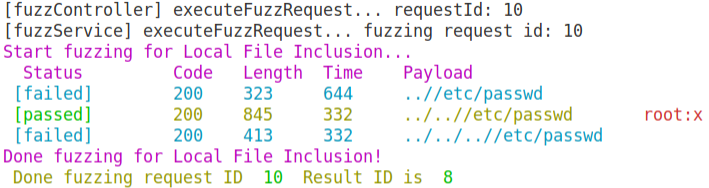
\includegraphics[width=\textwidth,keepaspectratio=true]{images/terminal-result.png}
  \caption{Kết quả kiểm thử trên terminal backend}
  \label{fig:terminal-result}
\end{figure}
Những payload phát hiện được lỗi (có xuất hiện các chuỗi khớp trong body hoặc thời gian thực thi request thỏa cấu hình kiểm thử) sẽ được đổi màu để làm nổi bật trên terminal như Hình \ref{fig:terminal-result}. Trong trường hợp trên, payload ``\texttt{../..//etc/passwd}'' khiến máy chủ web mục tiêu trả về response có body chứa chuỗi ``\texttt{root:x}'', dấu hiệu khai thác thành công lỗ hổng \acrshort{lfi}. Mỗi dòng kết quả này bao gồm các thành phần sau.
\begin{itemize}
  \item \textbf{Kết quả kiểm thử} được đặt trong cặp ngoặc vuông, có thể là \texttt{[passed]} trong trường hợp payload khai thác thành công lỗ hổng hoặc \texttt{[failed]} trong trường hợp payload không khai thác thành công.
  \item \textbf{Mã trạng thái HTTP} của response trả về, thường là \texttt{200} trong trường hợp request được gửi thành công hoặc các mã lỗi \texttt{401}, \texttt{404}, \texttt{500},... khi có sự cố trong quá trình xử lí request ở ứng dụng web mục tiêu.
  \item \textbf{Độ dài nội dung} của response trả về, \textbf{thời gian xử lí} của request tính theo giây, \textbf{payload} tương ứng được gửi theo request kèm theo những chuỗi khớp với cấu hình kiểm thử (nếu có).
\end{itemize}
\textbf{Mô-đun lưu trữ kết quả kiểm thử (\texttt{updateFuzzingLog})} sẽ lưu trữ những payload kèm theo loại lỗ hổng phát hiện được dựa trên kết quả kiểm thử trên. Những kết quả này được lưu lại dưới dạng chuỗi vào cơ sở dữ liệu theo cấu trúc như Đoạn mã \ref{lst:example-result} sau.
\begin{lstlisting}[style=ES6, label={lst:example-result}, caption={Cấu trúc kết quả kiểm thử}]
{
  "1": [
    {
      payload: '../..//etc/passwd',
      payloadIdx: '0',
      matchList: ['root:x'],
      timebased: false
    },
    ...
  ],
  ...
}
\end{lstlisting}
Kết quả kiểm thử sẽ được phân loại theo ID của mỗi loại lỗ hổng. Đối với mỗi payload phát hiện được lỗ hổng này, chúng tôi lưu trữ đầy đủ kết quả so trùng, thời gian thực thi request và vị trí chèn payload trên \acrshort{http} request mẫu, phục vụ việc trả kết quả về hiển thị trên \acrshort{ui} và hiện thực chức năng tái hiện request/response kiểm thử trong tương lai.